\chapter{Development}

\section{Hardware Design}
The hardware of the Reefing System was designed using Altium Designer 22. The integrated 3D \acrshort{cad} functionality simplified the overall development and lowered the possibility of errors in the design. The small footprint and consequently extremely dense placement of components required a 6-layer \acrfull{pcb}. The board, with the size of 50\,mm\;x\;35\,mm has been manufactured and assembled by JLCPCB.

\begin{figure}[h!]
	\hspace{-2.2cm}
	\includegraphics[height=11.0cm]{images/render1}
	\caption{Assembled PCB 3D-Render}
	\label{fig:rendering-pcb}
\end{figure}
\newpage

\subsection{Block Diagram}
The hardware block diagram in Figure \ref{fig:hardware-block-diagram} offers an overview of the system architecture. The complete schematic can be found in Appendix \ref{apx:schematic}.  

\medskip
\begin{figure}[h!]
	\centering
	\includegraphics[width=\textwidth]{images/block_diagram}
	\vspace{0.1cm}
	\caption{Hardware Block Diagram}
	\label{fig:hardware-block-diagram}
\end{figure}




\clearpage

\subsection{Microcontroller} \label{microcontroller}
The microcontroller is an essential part of any embedded system. It is the brain of the whole design, processing all incoming and outgoing data.  
\subsubsection{Selection}
Current shortages of chips essentially dictated the selection of a suitable microcontroller. Several factors were carefully considered and key requirements have been set, such as:

\begin{itemize}
		\item System performance: \acrshort{cpu} speed, memory and peripherals
		\item Native \acrshort{usb} 2.0 Interface
		\item Physical package and pin count
		\item Low power draw
		\item Stop mode to preserve battery life
		\item Availability
\end{itemize}

The best suitable \acrshort{mcu} family for the given requirements is the \gls{stm32}L4 ultra-low-power series. Their low power draw and high performance and the native USB 2.0 interface make them ideal for the application. Unfortunately, the availability of the low-power series microprocessors is terrible. Because of that, the decision was taken to go with an older, about as powerful but less efficient, \gls{stm32}F4 microprocessor. In particular, the STM32F411CC was chosen because they were available for assembly by JLCPCB.   

The \acrshort{mcu} selected is based on the high-performance ARM Cortex-M4 32-bit \acrshort{risc} core. Some of its features can be seen in the info graphic \ref{fig:coretex-m4}

\begin{figure}[h!]
	\centering
	\includegraphics[height=9cm]{images/cortrex-m4}
	\caption{ARM Cortex-M4 Block Diagram}
	\vspace{-1.4ex}
	\caption*{\textbf{Source:} ARM Developer Cortex-M4 Techical Specification \cite{arm-techspecs}}
	\label{fig:coretex-m4}
\end{figure}


\subsubsection{Programming and Debugging}
The \acrshort{mcu} can be programmed over Serial Wire with a suitable programmer (e.g., STMicoroeletronics ST-Link). Through the programmer, debugging is fully supported, allowing fast and efficient software development. 

\subsubsection{Clock Source}
The microprocessor supports clock frequencies up to 100\,MHz. By using an external 8\,MHz crystal oscillator, the main \acrshort{cpu} clock frequency can be adjusted according to the power and processing needs. Another key benefit of an external crystal oscillator is the temperature stability and accuracy of the clock source. However, these factors are not of great relevance for the application.

\subsection{Battery}
The reefing system is permanently attached to a battery. In order to prevent damage to the battery, systems are put in place to protect and monitor it. 

\subsubsection{Battery Selection}
The heating element consumes a lot of current when activated. In order to deliver the currents needed to cut the line, a \acrfull{lipo} battery was selected. In comparison to the more commonly used \acrshort{liion} batteries, \acrshort{lipo} batteries are more power-dense. Meaning they can deliver more current for their size and weight.

The C discharge rating of a battery determines how much current can be pulled from it without overheating. One C is equivalent to a fully charged battery being discharged in one hour. For example, a battery with a rating of 30\,C can dump the whole energy stored in just 2 minutes. The battery selected is a Swaytronic 650\,mAh one cell \acrshort{lipo} battery with a continuous C rating of 35. The battery can be safely discharged at 22.75A, providing enough margin for a successful deployment. 

\begin{figure}[h!]
	\centering
	\includegraphics[width=10cm]{images/swaytronic.jpg}
	\caption{Swaytronic 1S 3.7V 650mAh Battery}
	\vspace{-1.4ex}
	\caption*{\textbf{Source:} Swaytronic Webshop \cite{swaytronic}}
	\label{fig:swaytronic}
\end{figure}

\subsubsection{Battery Protection}
In order to protect the battery from under-voltage, over-voltage, and over-current, a battery management chip was selected. Two N-Channel \acrshort{mosfet} operated in a bi-directional switching configuration allow the battery protection \acrshort{ic} to shut off charging or discharging. Whenever the under-voltage threshold is reached, the discharging \acrshort{mosfet} is turned off, allowing the battery to be charged but not further discharged. While charging, as soon as the battery surpasses the minimum allowed voltage, the discharge \acrshort{mosfet} is turned back on. The same goes for an over-voltage event. In that case, charging is disabled, while discharging the battery is possible. 

The under- and over-voltage detection work by measuring the battery voltage directly. The over-current detection, on the other hand, measures the voltage drop across the two \acrshort{mosfet}. For the selected battery protection \acrshort{ic}, the maximum allowed voltage drop across the two \acrshort{mosfet} is 0.15\,V. As soon as that voltage is surpassed, the system gets cut off from the battery. A delay circuit inside the \acrshort{ic} turns the power back on after a short delay. 

\begin{figure}[h!]
	\centering
	\includegraphics[width=10cm]{images/battery-protection}
	\caption{Simplified Battery Protection}
	\label{fig:battery-protection}
\end{figure}

While cutting a reefing line, the system requires a large current. This current has to be lower than the current limit on the battery protection circuit. Therefore the system was designed to allow a current of at least 15\,A to flow. In order for the system to not trigger over-current events, low internal resistance \acrshort{mosfet} were selected. The Equation \ref{eq:mosfet} shows the maximum allowed internal drain-source resistance of a \acrshort{mosfet} while turned on.

\begin{equation}\label{eq:mosfet}
    R_{DS(ON)} = \frac{U}{2 \times I} = \frac{0.15V}{2 \times 15A} = 5m\Omega
\end{equation}

Initially, some problems with the battery protection circuit were experienced. The battery protection did not switch off whenever the battery voltage reached a critically low voltage, resulting in one of the batteries being deeply discharged. However, only two of the ten boards showed this behavior after much testing. Indication a problem with the assembly, the chip or the \acrshort{mosfet}. No further investigation was conducted.

\subsubsection{Battery Charging}
The battery can be charged through the \acrshort{usb} port on the reefing system. A charging \acrshort{ic} developed by \textit{MicrOne} was used to linearly regulate the 5\,V from the \acrshort{usb} to the battery voltage. The battery is being charged with a constant current until the maximum battery voltage of 4.2\,V is reached. Once the threshold voltage is reached, the charging chip switches to a constant voltage mode. The charging current slowly reaches zero up until the battery is fully charged. Figure \ref{fig:charging-curve} shows an example charge curve of a battery.

\begin{figure}[h!]
	\centering
	\includegraphics[width=10cm]{images/charge-curve}
	\caption{Example Charge Curve of Lithium Battery}
	\label{fig:charging-curve}
\end{figure}

The charge current can be programmed using a resistor between the \acrshort{ic}s \textit{PROG} pin and ground. Supported are currents of up to 800\,mA. A \acrshort{lipo} battery should not be charged with currents higher than 1\,C. Therefore, a battery with a capacity of 650\,mAh should only be charged with a maximum current of 650\,mA. In order to support a wide range of battery sizes, a jumper was placed on the board that adds a second resistor of the same size in parallel to the first one, doubling the charging current from 300\,mA to 600\,mA. 

\subsubsection{Battery Monitor}
The system can measure the battery voltage using a resistor divider and an analog input on the microcontroller. The voltage divider is built with large resistors, keeping the power dissipation low. A 100\,nF capacitor is used to smooth out the voltage going to the microcontroller. The battery voltage measurement can be reported to the user or used internally for power-saving operations.

\subsubsection{Connector}
Unfortunately, Wire-to-Board connectors rated for the expected currents require a large footprint. For that reason, the battery is soldered directly to the board, providing an extremely low resistance connection with the drawback of not being able to remove the battery quickly.

\newpage

\subsection{Power Management}\label{power-management}

The power management of the system is quite complex. Powering the device from the \acrshort{usb} port, keeping the power draw low while sleeping in addition to the high power draw while cutting, required some clever circuitry. Figure \ref{fig:pm} shows a simplified version of the power management.

\begin{figure}[h!]
	\centering
	\includegraphics[width=\textwidth]{images/pm}
	\caption{Simplified Power Management of the Reefing System}
	\label{fig:pm}
\end{figure}

\subsubsection{3.3V Power Rails}
In order to keep the power consumption low during sleep modes, multiple power rails were added. The primary power rail is generated from the input voltage using a \acrshort{dcdc} step-down converter. The main power rail, operating at 3.3\,V is connected only to the microcontroller and the sensors operating in low power modes. Two load switches prevent the primary power supply voltage from powering the rest of the system. One of the load switches is intended for all circuitry that powers the cutting mechanism. The second power rail is for the telemetry section. The load switches are operated from the microcontroller, allowing the software to control when each rail is on.

\subsubsection{Heating Element Power Supply}
A \acrshort{dcdc} step-up converter is used to drive the heating element. The TPS61088 is a fully-integrated synchronous boost converter intended for high-power portable applications. The \acrshort{ic} has a wide input voltage range and supports applications with single-cell or two-cell lithium batteries. Texas Instruments rates the \acrshort{ic} to deliver up to 3\,A at 12\,V for a short duration, making it ideal for driving the heating element. The \acrshort{dcdc} converters output voltage can also be adjusted from 4.5\,V to 12.6\,V using a resistor divider. In order to test different heating profiles, a digital potentiometer is used to change the output voltage. The voltage can be adjusted over the full range of the TPS61088 with a step size of around 30\,mV. The digital potentiometer is programmed using \acrshort{spi} and offers 256-taps. 

The \acrshort{dcdc} converter can be powered on and off using the \textit{EN} pin from the TPS61088. Additionally, the heating element can be switched using a power \acrshort{mosfet} allowing for continuous or \acrshort{pwm} operation.

\subsubsection{Ideal Diode and Charging}
While charging, the battery is disconnected from the main power rail, and the current from the \acrshort{usb} is used. This switching was done by using two diodes in parallel. For the battery side, the diode is inside a \acrshort{mosfet}, driven by the ideal diode controller. Resulting in a low voltage drop whenever the system is in flight. The ideal diode controller is turned off as soon as the USB is connected. In that case, the voltage from the USB is always greater than the voltage from the battery, allowing only current to flow from the USB port to the system. 

Unfortunately, the ideal diode controller selected is entirely unavailable for purchase. For that reason, the voltage from the \acrshort{dcdc} step-up converter was used to switch the \acrshort{mosfet}. This fix, which was added after the \acrshort{pcb}s were produced, is shown in Figure \ref{fig:pm} with a red line. With that change, the current consumption in run mode increases but has proven to be working as expected. While sleeping, the \acrshort{dcdc} step-up converter is shut off, allowing current to flow through the diode while preserving battery life. The step-up converter is also shut off immediately when a \acrshort{usb} cable is connected, preventing current from flowing backward into the battery.  

\subsection{Sensors}
\subsubsection{Inertial Measurement Unit}
A \acrfull{imu} was added to the board, intended for liftoff detection and to gather additional data during flight. The LSM6DSR is an ultra-low-power high-performance three-axis linear accelerometer and gyroscope with digital \acrshort{i2c}/\acrshort{spi} serial interface output. The accelerometer inside the sensor has user-selectable scales of ±2\,g up to ±16\,g and can measure with data rates from 1\,Hz up to 6.6\,kHz. The gyroscope has user-selectable scales of ±125\,dps up to ±4000\,dps and provides the same update rates as the accelerometer. The sleep modes provided have an ultra-low power consumption of less than 3\,$\mu$A. Additionally, wake-up on accelerometer action is available, allowing the system to sleep up to the point of rocket liftoff. The sensor is connected through \acrshort{spi} to the microcontroller.

\subsubsection{Barometer}\label{barometer}
A specialized barometric air pressure sensor is used to get altitude information. The sensor has an industry-leading range of 10 to 1200\,mbar allowing for altitude readings of up to around 30\,km above sea level. In addition, the barometer is advertised to have an extremely low power draw of 0.02\,$\mu$A when in standby. Unfortunately, during testing, it was noted that the barometer's current consumption was significantly higher. Contact with the manufacturer was established, but an explanation of that behavior is still pending. The sensor shares the \acrshort{spi} bus with the \acrshort{imu}.

\subsubsection{Thermocouple Interface}
A type-K thermocouple interface was added to monitor the temperature of the heating element. The MAX6675 is designed by Maxim integrated and consists of cold-junction temperature compensation, an analog-digital converter, and a \acrshort{spi} serial interface. The internal \acrshort{adc} with a range of 12\,bit provides a resolution of 0.25\,$^\circ$C and measures up to +1024\,$^\circ$C. Type-K thermocouples provide information about the difference in temperature between two ends of the wires. The cold end, which is the ambient temperature, can fluctuate. The MAX6675 senses and corrects for the changes in the ambient temperature with the cold-junction compensation.

\subsubsection{Light Sensor}
The light sensor is intended to detect the ejection of the parachute. The kind of light sensor used in this application is a phototransistor. In comparison to photodiodes, phototransistors have a much higher gain, allowing for minor light differences to be detected. The collector is connected to the cutting 3.3\,V power rail, reducing current consumption when not in use. The emitter of the sensors is directly connected to a microcontroller \acrshort{adc} pin and a 10\,k$\Omega$ resistor to ground.


\subsection{Telemetry}
The system should be capable of receiving telemetry from the main flight computer of the rocket. For that reason, the telemetry part of the hardware was mostly copied from the existing design of the \gls{cats} flight computer. The \gls{cats} flight computer is the main recovery computer used by \acrshort{aris} in their rockets. 

\begin{figure}[h!]
	\centering
	\includegraphics[width=10cm]{images/antenna}
	\caption{Telemetry Section, PCB view}
	\label{fig:antenna}
\end{figure}

\subsubsection{Microcontroller}
The telemetry has a dedicated microcontroller. The task of that microcontroller is to keep the radios synchronized without worrying about other processing tasks. An STM32G071GB was selected for its low price, small footprint, and availability. The \acrshort{mcu} provides no interface for an external crystal oscillator. Therefore the internal one was used. The time stability of the internal oscillator is sufficient to keep time synchronization between the transmitter and receiver.

\subsubsection{Radio}
The radio used for the telemetry link is a Semtech SX1280. It is a \acrshort{lora} 2.4\,GHz \acrshort{rf} transceiver that provides excellent range and low power consumption. An external 52\,MHz crystal oscillator is required, and its frequency gets boosted internally to the carrier frequency. The radio is connected over \acrshort{spi} to the telemetry \acrshort{mcu}. Additionally, two interrupt signals and the busy signal are used for more efficient operation.

\subsubsection{Impedance \& Filter}
The transmission line impedance of the \acrshort{rf} signal line is 50\,$\Omega$. Therefore, close attention was paid to match the \acrshort{pcb} trace to the target impedance by calculating the line thickness and distance to ground. An integrated Altium Designer tool was used for all calculations based on the stack-up of materials and rules added to the transmission lines.  

A \acrshort{ipc} 2.4\,GHz \acrshort{rf} filter was added to the board. A \acrfull{ipc} is a single surface mount component with a filter network built-in. Due to manufacturing and component tolerances, they require considerably less space on the board and often perform better than discrete filters. The main task of the low pass filter is to reduce the harmonics generated by the radio. The selected \acrshort{rf} filter from Johanson Technology matches the transmission line impedance of 50\,$\Omega$.  

\subsubsection{Antenna}
A PCB antenna was added to the board. The design was taken from the Texas Instruments application Note AN043 \cite{ti-antenna}. The antenna chosen has a small footprint and provides good performance. With a reflection of less than -10\,dB over the whole 2.4\,GHz frequency band, the design ensures efficiency of more than 90\,\%. The antenna is linearly polarized and has an omnidirectional radiation pattern. With a matching impedance of 50\,$\Omega$, the antenna requires no additional components on the board. The antenna design can be seen through the solder mask in Figure \ref{fig:antenna}.

\newpage
\section{Mechanical Design \& Line Cutter}

\subsection{Line Cutter}

\subsubsection{Specifications}
The ceramic heating element obtained from Aliexpress has an inner diameter of 4\,mm and an outer diameter of 6.6\,mm. The selected element has an operating voltage of 12\,V. The electrical resistance at room temperature is 8.2\,$\Omega$ and settles at around 18\,$\Omega$ when the maximum temperature of 450\,$^\circ$C is reached. Therefore the power supply needs to deliver a minimum current of 1.5\,A at 12\,V to heat the element quickly. The \acrshort{dcdc} converter, presented in Section \ref{power-management} fulfills this requirement. 

\subsubsection{Insulation}
The heating element needs to be thermally insulated not to burn its surroundings. In order to keep the heat contained, the element is wrapped in multiple layers of fiberglass insulation material. The insulation protects the enclosure from overheating and keeps the heat inside the element, speeding up the separation of the line. In addition, aluminum tape is wrapped around the fiberglass, keeping it in place and reflecting additional heat. The insulating barrier is about 5\,mm thick and keeps the temperatures on the outside below 50\,$^\circ$C after one minute of heating, providing enough margin for the enclosure and surrounding electronics to not be damaged.

\begin{figure}[h!]
	\centering
	\includegraphics[width=\textwidth]{images/heating-elemet}
	\caption{Open Enclosure with heating element and PCB inside}
	\label{fig:heating-element}
\end{figure}


\newpage

\subsection{Enclosure}
A case for the reefing system was designed using the \acrshort{cad} software SOLIDWORKS 2022. The enclosure is manufactured using a 3D printer. 

\begin{figure}[h!]
	\centering
	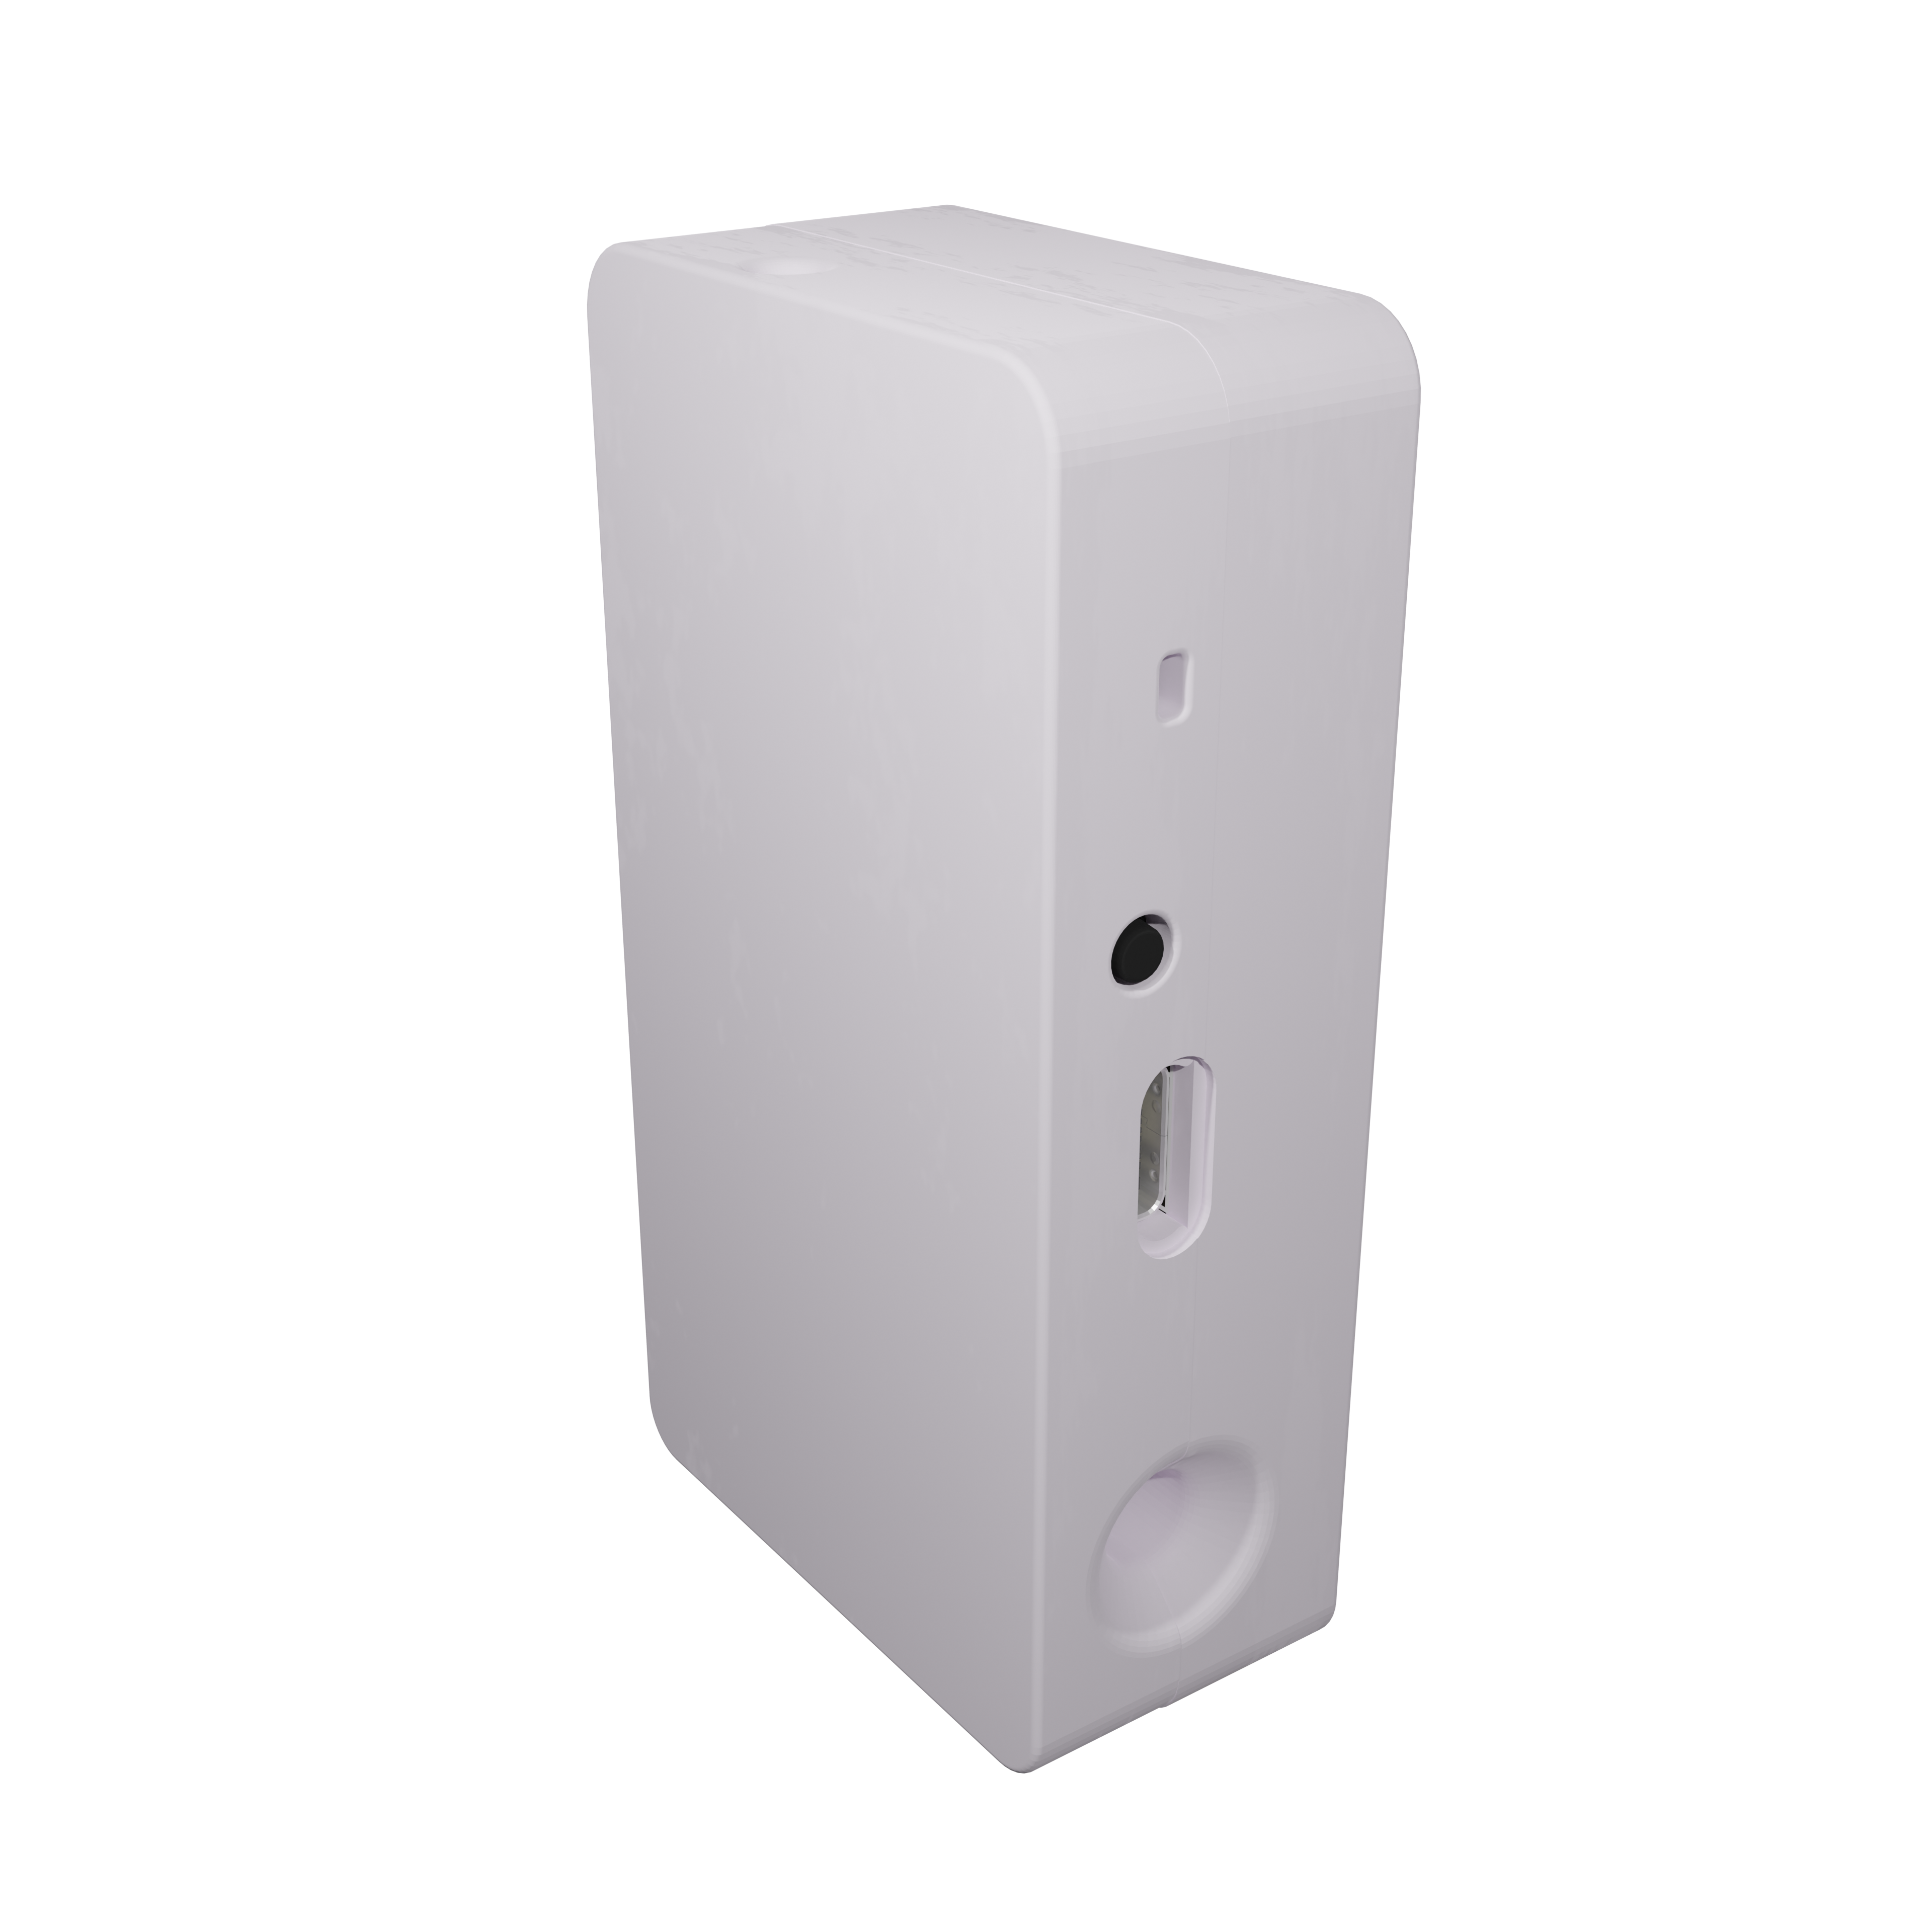
\includegraphics[width=8cm]{images/case}
	\caption{Enclosure 3D-Render}
	\label{fig:enclosure}
\end{figure}


\subsubsection{Design}
All parts, the PCB, battery, and heating element were imported into the \acrshort{cad} software in order to design an enclosure around it. The case is built from two halves, the bottom part where the battery and \acrshort{pcb} are mounted and the top part, where holes for the \acrshort{usb} connector and button are placed. A set of M3 screws are used to assemble the enclosure. Threaded inserts, added after printing, make it possible to open and close the case repeatedly. The heating element is clamped together, and channels guide the reefing line to the heating element. 

\subsubsection{Manufacturing}
Initial prototypes were printed using \acrshort{pla} plastic filament on a \acrshort{fdm} printer. \acrfull{fdm} is a method of additive manufacturing where layers of materials are fused together. The material is melted and then extruded in a pattern next to or on previous extrusions, creating an object layer by layer. The main advantage of this manufacturing process is the fast and cheap process. 

The final design is manufactured using LEDO 6060 plastic. Compared to the \acrshort{pla} plastic filament, it provides better dimensional stability and good temperature resistance. The parts are manufactured using a \acrfull{sla} printer. Other than the \acrshort{fdm} process, the printers use a light source to cure liquid resin into hardened plastic. JLCPCB manufactured the enclosure. They print the design on industrial-grade machines resulting in excellent surface finish and accuracy.

\newpage

%% Section Firmware %%
\section{Firmware}
The firmware is written in C and is based on the STMicroelectronics \acrshort{hal} libraries. As an \acrshort{ide}, CLion together with CubeMX is used. This modern environment ensures rapid and efficient development.\newline
FreeRTOS is the real-time operating system of choice. It guarantees a reliable operation and handles multi-task operations on single-core systems.

\subsection{Operation}\label{operation}

The state event diagram in Figure \ref{fig:fsm} offers an overview of the behavior of the system.

\begin{figure}[h!]
	\centering
	\includegraphics[width=\textwidth]{images/fsm}
	\caption{Finite State Machine}
	\label{fig:fsm}
\end{figure}

\subsubsection{Deep Sleep}
During deep sleep, the microcontroller is put into stop mode, all auxiliary power rails are turned off, and the sensors are put into sleep mode. During deep sleep, the power consumption is minimized to preserve battery life. In addition, all interrupts except for the button pin are turned off. Therefore the system can only be woken up by user input.  

\subsubsection{Idle}
When woken up from deep sleep, the system goes into idle mode. The user can configure the device through the USB port or check the battery life during this state. If the device is inactive for over a minute, it will automatically return to deep sleep. Before liftoff, with user input, the device can be put into ready mode.

\subsubsection{Ready}
In the ready state, both the barometer and accelerometer are constantly readout. The barometric air pressure data is used to calculate the altitude and passes through a Kalman filter. After 30 seconds, the microcontroller puts the accelerometer in wake-up mode and goes to stop mode—preserving battery life before the rocket's liftoff. An acceleration event triggers an interrupt and puts the microcontroller back into run mode. If the acceleration is greater than a user set threshold for over 100\,ms, the rocket's liftoff is detected. User input during the ready state can transition the finite state machine back into idle mode. 

\subsubsection{Ascent}
After liftoff is detected, the rocket ascends to apogee. The barometer is read out and passed through the state estimation during this phase. The estimated vertical velocity is used to detect the highest point in the flight. At that point, the vertical velocity hits zero and becomes negative. As soon as the velocity sign changes, the apogee is reached, and the finite state machine advances to the descent phase.

For short-duration flights, the heating element is getting preheated as soon as liftoff is detected. The temperature only slowly rises and does not damage the reefing line by applying a lower voltage to the element. Preheating is only recommended on very short flights if there is not enough time for the element to heat up between apogee and the main altitude. 

\subsubsection{Descent}
During the descent phase, the velocity and altitude are read out continuously. With the data obtained, the deployment altitude is calculated and initiates the separation as soon as the following criteria applies:
\begin{equation}
    h_{deploy} < (h + v \times t_{burn}) 
\end{equation}
where
\begin{itemize}
    \item $h_{deploy}$ is the user set deployment altitude in m;
    \item $h$ is the current altitude in m;
    \item $v$ is the current velocity in m/s;
    \item $t_{burn}$ is the estimated burn duration in s;
\end{itemize}

\subsubsection{Recovery}
After separating the lines, the system goes into recovery mode. The reefing system continuously beeps, making the recovery operation of the rocket easier. The device can be disabled with user input, returning to the idle state.

\newpage

\subsection{RTOS}
The system is running on FreeRTOS, an open-source, free-to-use \acrlong{rtos} developed by Real Time Engineers Ltd. The operating system runs with a tick rate of 1000\,Hz while most tasks operate at 100\,Hz. Seven tasks are running simultaneously while the system is in flight. The sensor readouts, state estimation, and finite state machine operate at 100\ Hz. Event-based tasks, like the buzzer, execute only once whenever requested. The health monitor, telemetry, and heater operate at a fixed frequency of 10\,Hz.

The \acrshort{rtos} is operated with preemption enabled, allowing task switching. All tasks are running with the same priority, preventing deadlocks but with the downside of slowing down the system if a task is blocked.   

\subsection{Sleep Mode}
As already described in Section \ref{operation} the microcontroller can be put in to stop mode to preserve battery life. The microcontroller is in the deepest possible sleep mode with memory retention in this operating state. All clock sources are turned off, and the low power regulator is used. From the datasheet, in this configuration, the current consumption of the \acrshort{mcu} is reduced to around 38\,$\mu$A. Outside the chip, all power rails, except for the main 3.3\,V supply, are turned off, and all sensors are put in standby mode. The only wake-up source in sleep mode are external interrupts. Only the button can wake the system up in the deep sleep state. While during the ready state, both the button and the accelerometer interrupt can return the \acrshort{mcu} from stop mode.  

According to some calculations ahead of time, the power consumption of the whole system in deep sleep mode should not exceed 100\,$\mu$A. But unfortunately, the measured current is a lot higher. As explained in Section \ref{barometer}, the main cooperate for the high consumption is the barometer. All current measurements were done using the NORDIC Semiconductors Power Profiler Kit II. The 200\,nA to 1\,A range made it possible to monitor the power consumption accurately.  

\begin{figure}[h!]
	\includegraphics[width=\textwidth]{images/current}
	\caption{Current measurements with the Power Profiler II}
	\label{fig:current}
\end{figure}

\subsection{Telemetry}

For the system to receive commands from the main flight computer of the rocket, the telemetry system is designed to be compatible. The telemetry link on the main fight computer of the rocket is based around \acrlong{fhss} and was developed by the author.

\subsubsection{Hopping Pattern}
The hopping pattern is defined with a password. The password is hashed using a \acrshort{crc}32 algorithm, and the resulting \acrshort{crc} is then used as the seed for a pseudo-random number generator. The generator is run 20 times, defining the hopping pattern. With this method, a password always generates the same hopping pattern. Both the transmitter and receiver require the same password for the transmission to work.

\subsubsection{Synchronization}
The receiver waits on the first frequency until a sync packet is received. The sync packet contains the link \acrshort{crc} to identify the transmission source. If the remote \acrshort{crc} matches the local \acrshort{crc}, the receiver hops to the subsequent frequency, waiting for data. Each data package contains a checksum to validate the contents. The time between packages is measured and used to jump to the next frequency when no package was received in the estimated time frame. A total of 30 hops can be performed without receiving a package before the synchronization is lost. On connection loss, the receiver returns to the first frequency.  

\subsubsection{Package}
Each package contains 14\,Bytes of data but only the state, altitude, and velocity are relevant for the Reefing System. The data is squashed as much as possible to maximize throughput and range.

\begin{figure}[h!]
	\includegraphics[width=\textwidth]{images/package}
	\caption{Telemetry Data from main flight computer of rocket}
	\label{fig:rf-package}
\end{figure}

\subsubsection{Future use}
Since the main flight computer of the rocket is also still in development and the data is not to be 100\,\% trusted, the Reefing System is only operating in independent mode, meaning the telemetry data is not used at all during flight. However, the device can interface with the main flight computer and use its data for all aspects of flight in the future. 

\subsection{Data Logger}
In order to validate the system and replay flight data, an onboard logging system was added. Since the device is always powered, data is being logged into the \acrshort{ram} of the main \acrshort{mcu}. Each element logged has a size of 5\,B containing the type of data, a timestamp in ms, and the recorded data. With a total reserved size of 64\,kB, it is possible to log 12800 elements per flight.

Only one flight can be recorded on the device. When the system detects liftoff, the previously stored data is overwritten. As soon as the allocated \acrshort{ram} is filled up, the recording is stopped, preventing overflows.  

Four different logging elements were added: the filtered altitude, the estimated altitude, the estimated velocity, and the state transitions. While altitude and velocity data are logged in every user-configured iteration, the state transitions are only logged whenever they occur. 

Maximum log durations of 42 seconds are possible when logging at full speed. The time can be extended for longer flights by changing the logging interval. This can be done through the USB port as explained in Section \ref{usb}.

The logged data can be read out through the \acrshort{usb} port and is then parsed with a jupyter notebook. Using pandas, the data is scaled to \acrshort{si} units and plotly to visualize the recorded flight. Plotly generates interactive plots, allowing for efficient data analysis.

\begin{figure}[h!]
	\includegraphics[width=\textwidth]{images/plotly}
	\caption{Visualization of rocket altitude using plotly}
	\label{fig:plotly}
\end{figure}

\newpage

\subsection{USB}\label{usb}
The \acrshort{usb} interface is initialized as a \acrfull{vcp} using the provided libraries from STMicroelectronics. When opening the serial port in a terminal, the device provides diagnostics and battery voltage information. Additionally, it provides a \acrfull{cli} to configure settings on the device, read out data logs, and get general information about the device. The following commands are implemented on the system as presented by the \acrshort{cli}.


\bigskip
\colorlet{mygray}{black!30}
\colorlet{mygreen}{green!60!blue}
\colorlet{mymauve}{red!60!blue}
\begin{lstlisting}[backgroundcolor=\color{gray!10},  
                   basicstyle=\ttfamily,
                   columns=fullflexible,
                   breakatwhitespace=false,      
                   breaklines=true,                
                   captionpos=b,                    
                   commentstyle=\color{mygreen}, 
                   extendedchars=true,              
                   frame=single,                   
                   keepspaces=true,             
                   keywordstyle=\color{blue},      
                   language=C,              
                   numbers=none,                
                   numbersep=5pt,                   
                   numberstyle=\color{blue}, 
                   rulecolor=\color{mygray},        
                   showspaces=false,
                   showstringspaces=false,
                   showtabs=false,                 
                   stepnumber=5,                  
                   stringstyle=\color{mymauve},    
                   tabsize=2,                      
                   title=\lstname,
                   frame=none,
                   xleftmargin = 1cm,
                   framexleftmargin = 1em]
>help
defaults - reset settings to defaults
dump - dump full configuration
get - get variable value
        [cmd_name]
help - display command help
log_enable - enable the logging output
reboot - reboot system
read - print out last recorded flight
save - save configuration
set - change setting
        [<cmd_name>=<value>]
status - show status
version - show version

>

\end{lstlisting}

All configurable settings are shown in the example below. Some of the most important settings are the acceleration threshold used to define the sensitivity of the liftoff detection, the heating element burn duration, and the main altitude. 

\bigskip
\colorlet{mygray}{black!30}
\colorlet{mygreen}{green!60!blue}
\colorlet{mymauve}{red!60!blue}
\begin{lstlisting}[backgroundcolor=\color{gray!10},  
                   basicstyle=\ttfamily,
                   columns=fullflexible,
                   breakatwhitespace=false,      
                   breaklines=true,                
                   captionpos=b,                    
                   commentstyle=\color{mygreen}, 
                   extendedchars=true,              
                   frame=single,                   
                   keepspaces=true,             
                   keywordstyle=\color{blue},      
                   language=C,              
                   numbers=none,                
                   numbersep=5pt,                   
                   numberstyle=\color{blue}, 
                   rulecolor=\color{mygray},        
                   showspaces=false,
                   showstringspaces=false,
                   showtabs=false,                 
                   stepnumber=5,                  
                   stringstyle=\color{mymauve},    
                   tabsize=2,                      
                   title=\lstname,
                   frame=none,
                   xleftmargin = 1cm,
                   framexleftmargin = 1em]
>set
Current settings:
acc_threshold = 35 m/s^2
main_altitude = 100 m
enable_telemetry = 0
enable_preheat = 1
buzzer_volume = 100 %
log_every_n = 5 samples
burn_duration = 35 s
link_phrase = -

>
\end{lstlisting}

The \acrlong{cli} was taken and adapted from the open-source project \gls{betaflight}.

\newpage

\subsection{Persistent Storage}
In order to store configuration settings and retain the information even after a reset, the onboard flash memory is used. The sectors of the microcontroller are not of equal length, therefore the flash mapping was modified to have the user configuration in two dedicated flash sectors each with a length of 16\,kB. As a result, the flash mapping is divided into the following partitions as shown in Table \ref{tab:Flash-Partitions}.

\begin{table}[h]
    \begin{tabular}{ | m{3.15cm} | m{3.7cm}| m{3cm} | m{2.5cm} |} 
      \hline
      \multicolumn{1}{|c|}{\textbf{Name}} & \multicolumn{1}{c|}{\textbf{Type}} & \multicolumn{1}{c|}{\textbf{Memory Address}} & \multicolumn{1}{c|}{\textbf{Size}}\\ \hline
      flash-startup & Startup code and Interrupt Vector Table & \codeword{0x8000000} & 16k \\ \hline
      flash-config & User configuration & \codeword{0x8004000} & 32k \\  \hline
      flash-app & Application & \codeword{0x800C000} & 464k \\  \hline
    \end{tabular}
    \caption{\label{tab:Flash-Partitions}Flash Partitions}
\end{table}

The implementation for reading and writing to the flash is straightforward. Each variable has a fixed length of 32\,bit and is stored with a virtual address, starting at zero. The virtual address is then mapped to the flash memory. In order to change a variable, the whole flash sector needs to be erased and then all stored variables are rewritten. Since the device's configuration is only changed a handful of times, no wear leveling is implemented. Despite contemplation, the implementation of a \acrfull{crc} was not carried out due to time constraints.

\subsection{Sensors}
All sensors on the board are read out, but not all of them are used for the operation. 

\subsubsection{Inertial Measurement Unit}
Only the accelerometer of the \acrshort{imu} is read out, as it is the only data needed for the operation. The maximum acceleration range of 16\,g is selected, and data is read out with a rate of 100\,Hz. Before liftoff, the sensor is put in sleep mode. Acceleration events above 1.5\,g wake the sensor up and generate an interrupt signal for the main microcontroller.

The sensor is used to detect the liftoff of the rocket. If the acceleration on the device is above a user set threshold for over 100\,ms, the finite state machine advances to the ascent phase of the flight. From that point onward, the sensor is not used anymore. 

\subsubsection{Barometer}
The barometer provides accurate pressure and temperature data of the environment. The sensor only provides either the temperature or pressure data for each sample. Therefore the sensor is sampled at a rate of 200\,Hz. Alternating between the temperature and pressure readouts. 

The pressure data is used for the state estimation as explained in Section \ref{state-estimation}.

\newpage

\subsubsection{Thermocouple}
Over \acrshort{spi} the temperature of the thermocouple is readout. 

Initially, the idea of the sensor was to read the temperature of the heating element and build a controller around it. Unfortunately, the thermocouple placement turned out to be extremely difficult, and the temperature measured did not reflect the actual temperature of the heating element. Each device would need to be calibrated for an accurate temperature readout, and a displacement of the thermocouple would result in bad measurements. For that reason, the thermocouple is not used in the software.  

\subsubsection{Light Sensor}
A light sensor implementation was added, where the sensor can be used as a binary signal. The analog value from the sensor is converted using the microcontrollers \acrshort{adc}. 

Before ejection of the parachute, the Reefing System is in the dark. In that state, the sensor can be calibrated to detect a change in brightness. The change translates to the ejection of the parachute and can be used for the finite state machine. As of now, the sensor is not taken into account by the \acrshort{fsm}.

\subsection{State Estimation}\label{state-estimation}
In order to get accurate altitude and vertical velocity information, a state estimation is implemented. The Figure \ref{fig:state-est} provides an overview of the data flow.
\begin{figure}[h!]
	\includegraphics[width=\textwidth]{images/state-est}
	\caption{Overview of State Estimation Data Flow}
	\label{fig:state-est}
\end{figure}

\subsubsection{Moving Average}
The only sensor used for the state estimation is the barometer. In order to smooth out the data before passing it on, a moving average filter is implemented. For the filter, $k$ samples are summed up and then divided by their size $k$. The mean over the last $k$ data-points is denoted as $SMA_{k}$ and calculated as:

\begin{equation}
    SMA_{k} = \frac{1}{k}\sum _{i=n-k+1}^{n}p_{i}
\end{equation}

A filter size of 8 was chosen, as it is ideal for efficient operation. The division needed can be replaced with right shift operations on the hardware as the data is stored as an unsigned integer.

\subsubsection{Measurement}
The barometric air pressure is converted to the altitude above ground level. Because weather conditions affect altitude calculations, the pressure and temperature at sea level must be known. Since that data is not available, the \acrshort{icao} Standard Atmosphere model is used to calculate the relative altitude from liftoff. \acrshort{icao} defines the air temperature to be 15\,$^{\circ}$C below an altitude of 11\,km. Before liftoff, the system continuously takes air pressure readings, averages them, and stores it as the initial air pressure $P_0$. Using the barometric formula, the relative altitude can be calculated.\cite{atmosphere}

\begin{equation}
    h = \frac{T_0}{L}\times{}\left({\frac{P}{P_0}}^{\frac{-R\times L}{g\times M}} - 1\right)
\end{equation}

where
\begin{itemize}
    \item $h$ is the relative altitude in m;
    \item $T_0$ is the air temperature at sea level in K;
    \item $L$ is the standard temperature lapse $= -0.0065\frac{K}{m}$;
    \item $P$ is the current air pressure in Pa;
    \item $P_0$ is the air pressure at liftoff altitude in Pa;
    \item $R$ is the universal gas constant $= 8.31432 \frac{Nm}{molK}$;
    \item $g$ is the gravitational constant $= 9.81 \frac{m}{s^2}$;
    \item $M$ is the molar mass of Earth's air $= 0.0289644 \frac{kg}{mol}$.
\end{itemize}

Before passing the air pressure data through the formula, it is converted into a 32-bit floating-point number.

\subsubsection{Rate limiter}
In order to eject parachutes from a rocket body, the section where the parachute, and consequently the Reefing System, is located gets pressurized. These pressure spikes usually last for one to two seconds. For that reason, a rate limiter is implemented. The rate limiter prevents the altitude from dropping suddenly, thus preventing the Kalman filter from receiving bad data points. An implementation of a median filter was considered, but since the pressure spikes can last multiple seconds, it was decided against that option. 

Rockets can reach incredibly high speeds while ascending. Therefore the ascent rate is not limited by the rate limiter. For the descent, on the other hand, the rate limiter is set to -25\,m/s. In a nominal flight, descent rates will never surpass that threshold. Therefore, if the measured descent rate is less than the falling slew rate of -25\,m/s the output is calculated as:

\begin{equation}
    y(i) = \Delta t \times F + y(i-1) 
\end{equation}

where

\begin{itemize}
    \item $F$ is the falling slew rate;
    \item $\Delta t$ is time between samples;
\end{itemize}

\newpage

\subsubsection{Kalman Filter Design}

Kalman filters are used to estimate states based on linear dynamical systems. In order to estimate the current altitude and vertical velocity of the rocket a linear Kalman Filter was deployed. The state space of the filter is described as follows:
\begin{equation}
    x = \begin{bmatrix}h\\v\end{bmatrix}
\end{equation}
where
\begin{itemize}
    \item $h$ is the position (altitude) of the rocket;
    \item $v$ is the velocity of the rocket which can also be described as the derivative of the position $\dot{h}$.
\end{itemize}

We assume that between the previous $(k-1)$ and the current timestep $k$ constant accelerations $w_a$ act upon the rocket. The acceleration is normally distributed, with mean 0 and standard deviation $w_R \sim \mathcal{N} (0, \sigma_R)$. This process noise is used to tune the dynamics of the filter, which was done using a simulation and flight data of previous rocket flights. More information can be found in Section \ref{filter-tuning}.

From Newton's laws of motion we can conclude that:

\begin{equation}
    \dot{x} = Ax + Gw_a
\end{equation}

\begin{equation}
    \dot{x} = \begin{bmatrix}v\\a\end{bmatrix} =  \begin{bmatrix}0 & 1\\ 0 & 0\end{bmatrix} \begin{bmatrix}h\\v\end{bmatrix} + \begin{bmatrix}0\\1\end{bmatrix}w_a
\end{equation}

Since no control inputs are known, the model is simplified by removing the $B$ matrix.

For the measurement model we assume a Gaussian white noise for the sensor noise $w_R \sim \mathcal{N} (0, \sigma_R)$.
The measurement model is defined as:
\begin{equation}
    z = Hx + w_R
\end{equation}
\begin{equation}
    z = \begin{bmatrix}1 & 0\end{bmatrix} \begin{bmatrix}h\\v\end{bmatrix} + w_R
\end{equation}

Afterward, the model was discretized and implemented on the hardware. The discretization process and implementation can be found in Appendix \ref{apx:kalman}
